% =====================================================================
% פרק 4 — ניתוח השוואתי: ארה״ב 2007/08, ספרד 2007/08 וישראל 2022–2026
% RESEARCH_CORE_AGENT (Agent 2)
% =====================================================================
\chapter{ניתוח השוואתי: ארה״ב, ספרד וישראל}
\label{ch:comparative}

\begin{managerbox}
השאלה אם ישראל ״חוזרת על \en{2008}״ היא שאלה של מנגנונים ולא של דמיון כללי. מנהל בבנק, ביזמות או ברגולציה צריך לדעת אילו מנגנוני כשל של ארה״ב ושל ספרד קיימים בישראל, באיזו עוצמה, ואילו בלמים מוסדיים חסרו שם וקיימים כאן. פרק זה משווה את שלושת המקרים לפי אותם פרמטרים, ומכוון את מבחני הקיצון שבפרק~\ref{ch:delivery-wall} לנקודות התורפה.
\end{managerbox}

\section{מסגרת ההשוואה וטבלת הפרמטרים}
\label{sec:ch4-table}

ההשוואה מפורקת לממדים התואמים את מנגנוני הכשל שבטבלה~\ref{tab:ch2-mechanisms}: מבנה המוצר וזעזוע התשלום, מינוף משקי הבית, מינוף היזמים, מבנה המימון של הבנקים ורשתות הביטחון המוסדיות. נתונים רשמיים מוצגים עם מקור; ערכים מכוילים (מסוגננים, לסדר גודל) מסומנים בכוכבית ומשמשים להמחשה בלבד. טבלה~\ref{tab:ch4-comparison} מרכזת את שלושת המקרים לפי עשרה פרמטרים: ישראל דומה לארה״ב רק בדחיית מבחן היכולת של הרוכש, ולספרד בממד היזמי והבנקאי, ושונה משתיהן במינוף משקי הבית, באיגוח וברגולציה.

\begin{table}[!htb]
\centering
\caption[השוואה רב־פרמטרית: ארה״ב, ספרד וישראל]{השוואה רב־פרמטרית: ארה״ב \en{2007/08}, ספרד \en{2007/08} וישראל \en{2022–2026}}
\label{tab:ch4-comparison}
\small
\begin{tabularx}{\tabmaxwidth}{>{\raggedleft\arraybackslash}p{2.6cm} R R R}
\toprule
\hd{פרמטר} & \hd{ארה״ב \en{2007/08}} & \hd{ספרד \en{2007/08}} & \hd{ישראל \en{2022–2026}} \\
\midrule
מוצר דחיית התשלום & \en{Teaser/ARM}, \en{Interest-Only} \cite{fcic2011} & משכנתאות בריבית משתנה; אין מוצר דחייה ייחודי \cite{akin2014} & \deal{20/80}, \deal{20/50/30}, בלון במימון היזם \cite{boi_circular2816} \\
\midrule
מפעיל הזעזוע & איפוס ריבית ועצירת המימון מחדש \cite{mayer2009} & אבטלה וירידת מחירים \cite{akin2014} & משכנתא בריבית ובשמאות של יום המסירה \cite{boi2026_resloans} \\
\midrule
מגבלות \en{LTV/PTI} & חלשות; תיעוד חסר נפוץ \cite{mayer2009} & -- & \en{LTV} עד \pct{75}; \en{PTI} עד \pct{50} \cite{boi_directive329} \\
\midrule
חוב משקי הבית לתוצר & \pct{98.4} (\en{2007Q4}) \cite{bis_hhdebt} & כ־\pct{82}* & \pct{42.5} (\en{2025}) \cite{bis_hhdebt} \\
\midrule
\en{LTV} אפקטיבי & \pct{95}* & \pct{85}* & \pct{85}* \\
\midrule
חשיפת האשראי הבנקאי לנדל״ן & \pct{55}* & \pct{60}* & \pct{39} מהאשראי העסקי \cite{boi2026_recredit} \\
\midrule
מינוף המתווכים & בנקי השקעות עד \en{40:1} \cite{fcic2011} & קופות חיסכון אזוריות \cite{akin2014} & מאזן בנקאי מפוקח \cite{boi2026_recredit} \\
\midrule
מבנה המימון & הפקה לשם הפצה, \en{MBS/CDO} \cite{keys2010} & בעיקר במאזן \cite{akin2014} & במאזן; חוק איגוח טרם הושלם \cite{boi_survey2025,hapoalim_q3_2026} \\
\midrule
חבות הלווה & \en{Non-Recourse} בחלק מהמדינות \cite{ghent2011} & -- & חבות אישית מלאה (פרק~\ref{ch:israel}) \\
\midrule
עלות המשבר למערכת & כ־\en{4} מיליון משפחות איבדו את ביתן \cite{fcic2011} & \en{€60.6} מיליארד (\pct{5.6} תוצר) \cite{bde2017note} & טרם התממש \\
\bottomrule
\end{tabularx}

\vspace{2pt}
{\footnotesize * ערך מכויל ומסוגנן (להמחשה), אינו נתון נצפה; ״--״: לא נמצא נתון מאומת.}
\end{table}

\section{ניתוח המנגנונים}
\label{sec:ch4-mechanisms}

\paragraph{זעזוע התשלום: \en{Teaser/ARM} מול \deal{20/80}.}\label{subsec:ch4-shock}
המכנה המשותף של מוצרי ה־\en{Teaser/ARM} ושל מבצעי המימון הוא דחיית מבחן היכולת. בארה״ב כרבע מהמשכנתאות במחצית הראשונה של \en{2005} היו ״ריבית בלבד״ \cite{fcic2011}. בישראל הפער הממוצע בין חתימת העסקה לנטילת המשכנתא התרחב מכחצי שנה בשנים \en{2018–2022} לכשמונה חודשים ב־\en{2025}, בין היתר בעקבות תמריצי המימון של היזמים \cite{boi2026_resloans}.

עם זאת, קיימים שני הבדלים מהותיים. ראשית, בארה״ב הלווה כבר החזיק במשכנתא והזעזוע נבע מאיפוס הריבית, ואילו בישראל הרוכש ייבחן במבחני הוראה \en{329} (סעיף~\ref{sec:ch3-baseline}) ביום המסירה: המבחן נדחה אך לא בוטל. שנית, מאייר, פנס ושרלונד מראים כי עד אמצע \en{2008} המוצרים הלא־קונבנציונליים לא היו גורם מרכזי לחדלות הפירעון; הגורמים העיקריים היו ירידת המחירים והידרדרות החיתום \cite{mayer2009}. מכאן שהסיכון בישראל אינו במבנה המבצע עצמו, אלא באפשרות שביום המסירה המימון לא יהיה זמין בתנאים הדרושים. בתרחיש להמחשה, ההחזר החודשי עולה בכ־\pct{29} באיפוס \en{Teaser} ובכ־\pct{76} במעבר מתשלום ריבית בלבד במבנה \deal{20/50/30} למשכנתא מלאה (איור~\ref{fig:payment-shock}).

\paragraph{מינוף משקי הבית ומינוף נסתר.}\label{sec:ch4-hidden}
חוב משקי הבית ביחס לתוצר בישראל נמוך ממחצית רמתו בארה״ב ב־\en{2007} (טבלה~\ref{tab:ch4-comparison}). בארה״ב חוב זה היה ערוץ ההעברה המרכזי ממשבר הדיור לכלכלה הריאלית \cite{mian2009,mian2014}, ובישראל ערוץ זה חלש בהרבה. אולם המינוף המצרפי עשוי להסתיר מינוף גבוה ברמת העסקה. איור~\ref{fig:ch4-comparative-risk} מראה שה־\en{LTV} המדווח בישראל נמוך משל ארה״ב וספרד, אך ה־\en{LTV} האפקטיבי, המחושב על המחיר הכלכלי ולא על מחיר המחירון, מתקרב לרמה הספרדית. בתרחיש המחקר, משכנתא של \pct{75} על דירה שמחירה הכלכלי נמוך בכ־\pct{12} ממחיר המחירון (משוואה~\ref{eq:ch5-npv}) שקולה ל־\en{LTV} אפקטיבי של כ־\pct{85} (\en{0.75/0.88}). כל הערכים באיור מכוילים, למעט יחס החוב לתוצר בארה״ב ובישראל וחשיפת הבנקים בישראל.

\begin{figure}[!htb]
\centering
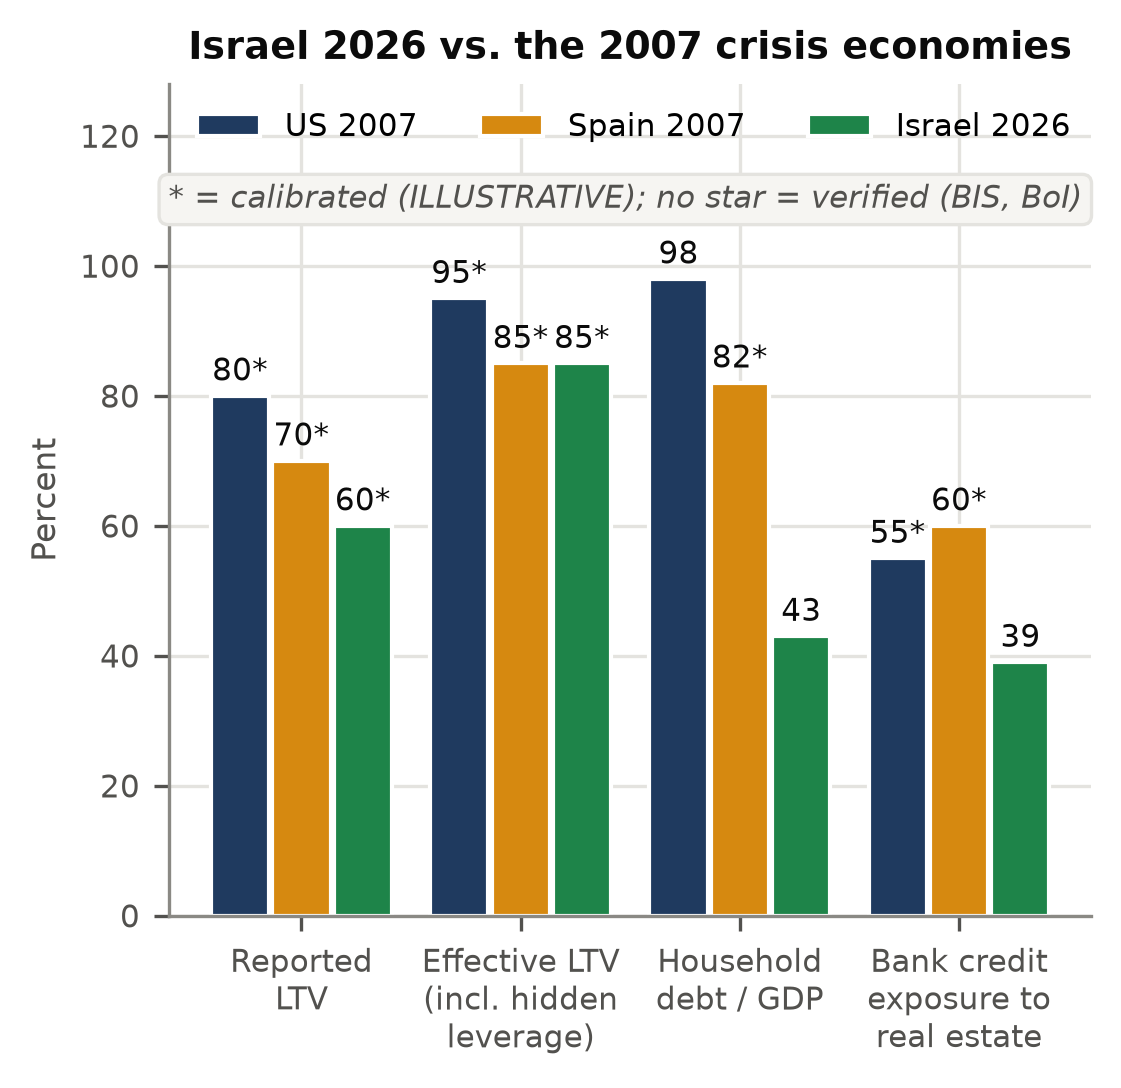
\includegraphics[width=0.65\textwidth]{figures/fig6_comparative_risk_2008_vs_2026.png}
\caption[השוואת מדדי סיכון: ארה״ב וספרד \en{2007} מול ישראל \en{2026}]{השוואת מדדי סיכון: ארה״ב \en{2007}, ספרד \en{2007} וישראל \en{2026}. ערכים המסומנים בכוכבית מכוילים להמחשה; החוב לתוצר בארה״ב ובישראל לפי \en{BIS}, וחשיפת הבנקים בישראל לפי בנק ישראל}
\label{fig:ch4-comparative-risk}
\end{figure}

\paragraph{מינוף היזמים וחשיפת הבנקים: הקבלה לספרד.}\label{subsec:ch4-developers}
בממד היזמי ספרד היא נקודת ההשוואה הקרובה ביותר: האשראי לבינוי ולנדל״ן הוזרם בעיקר דרך קופות החיסכון, ומשבר הנדל״ן הפך למשבר בנקאי גם ללא מוצרי משכנתא אקזוטיים \cite{akin2014}, בעלות משאבים נטו (ציבוריים ופרטיים) של כ־\en{€60.6} מיליארד (\pct{5.6} מהתוצר) עד סוף \en{2015} \cite{bde2017note}. בישראל, האשראי לענף הבינוי והנדל״ן מהווה כ־\pct{39} מהאשראי העסקי המאזני וכ־\pct{21} מהאשראי לציבור, והוא צמח ב־\en{2025} בכ־\pct{14} (האשראי לפרויקטים למגורים: כ־\pct{40}) \cite{boi2026_recredit}. זהו המנגנון שאפיין את ספרד: בנייה שמקדימה את המכירות ובנקים שחשיפתם לענף גדלה. ההבדל הוא במבנה: האשראי לפרויקטים ניתן בליווי סגור. אולם גם בישראל האשראי לקרקע למגורים (\nis{81} מיליארד, סוף \en{2025}) גדול מהאשראי לפרויקטים (\nis{69} מיליארד) \cite{boi_survey2025}.

\paragraph{מבנה המימון ורשתות הביטחון.}\label{subsec:ch4-safety}
בארה״ב ניתק מודל ״ההפקה לשם הפצה״ את המלווה מהסיכון \cite{keys2010}, ובנקי ההשקעות פעלו במינוף של עד \en{40:1} \cite{fcic2011}. בישראל האשראי מוחזק במאזני הבנקים: התמריץ לחתום בקפדנות נשמר, אך הסיכון מרוכז במערכת הבנקאית, כמו בספרד. שלושה בלמים מוסדיים מבדילים את ישראל. \textbf{חבות הלווה}: גנט וקודליאק מצאו שבמדינות ללא חבות אישית לווים נטו יותר לחדלות פירעון \cite{ghent2011}; בישראל החבות מלאה, ולכן ״פירעון אסטרטגי״ אינו צפוי. \textbf{ערבויות חוק המכר} מגנות על הרוכש מפני קריסת היזם \cite{salelaw1974}, אך מעבירות את הסיכון לבנק הערב, וערוץ זה נכלל במבחן הקיצון (משוואה~\ref{eq:ch5-coverage}). \textbf{מדיניות מאקרו־יציבותית}: ההפרשות הדינמיות בספרד מיתנו את מחזור האשראי \cite{jimenez2017} אך לא מנעו את המשבר \cite{bde2017}; בישראל פועלות הוראה \en{329} וחוזר \en{2816} (סעיפים~\ref{sec:ch3-baseline} ו־\ref{sec:ch3-boi}). הלקח הספרדי הוא שכלים אלה מצמצמים את הנזק, אך אינם מחליפים הגבלה של ריכוז החשיפה לענף אחד.

\section{מפת השחזור}
\label{sec:ch4-replication}

איור~\ref{fig:ch4-radar} מסכם את ההשוואה במפת עוצמה של שישה מנגנוני כשל, בסולם \en{1} (חלש) עד \en{5} (חזק). הציונים הם הערכה איכותית של צוות המחקר על בסיס טבלה~\ref{tab:ch4-comparison}, ולא מדידה. הפרופיל הישראלי חופף לספרדי בצד היזמי והבנקאי, לאמריקאי רק בדחיית מבחן היכולת, ונמוך משניהם בסיכון מחוץ למאזן ובחולשת הרגולציה.

\begin{figure}[!htb]
\centering
\begin{english}
\begin{tikzpicture}[scale=0.8, font=\footnotesize]
  \foreach \r in {1,...,5}{
    \draw[gray!35] (90:\r*0.5) -- (30:\r*0.5) -- (-30:\r*0.5) -- (-90:\r*0.5) -- (-150:\r*0.5) -- (150:\r*0.5) -- cycle;
  }
  \foreach \a in {90,30,-30,-90,-150,150}{ \draw[gray!50] (0,0) -- (\a:2.5); }
  \foreach \r in {1,...,5}{ \node[gray, font=\scriptsize, anchor=west] at (0.05,\r*0.5) {\r}; }
  \node[anchor=south] at (90:2.6) {\he{דחיית מבחן היכולת}};
  \node[anchor=west]  at (30:2.6) {\he{מינוף משקי הבית}};
  \node[anchor=west]  at (-30:2.6) {\he{מינוף יזמים ומלאי}};
  \node[anchor=north] at (-90:2.6) {\he{ריכוז חשיפת הבנקים}};
  \node[anchor=east]  at (-150:2.6) {\he{סיכון מחוץ למאזן}};
  \node[anchor=east]  at (150:2.6) {\he{חולשת רגולציה}};
  \draw[brandNavy, line width=1.2pt, fill=brandNavy, fill opacity=0.08]
    (90:5*0.5) -- (30:5*0.5) -- (-30:3*0.5) -- (-90:3*0.5) -- (-150:5*0.5) -- (150:5*0.5) -- cycle;
  \draw[brandAmber, line width=1.2pt, dashed, fill=brandAmber, fill opacity=0.08]
    (90:2*0.5) -- (30:4*0.5) -- (-30:5*0.5) -- (-90:5*0.5) -- (-150:3*0.5) -- (150:3*0.5) -- cycle;
  \draw[brandGreen, line width=1.4pt, fill=brandGreen, fill opacity=0.12]
    (90:4*0.5) -- (30:2*0.5) -- (-30:4*0.5) -- (-90:4*0.5) -- (-150:1*0.5) -- (150:1*0.5) -- cycle;
  \begin{scope}[shift={(-5.2,-3.55)}]
    \draw[brandNavy, line width=1.2pt] (0,0) -- (0.6,0); \node[anchor=west] at (0.75,0) {US 2007/08};
    \draw[brandAmber, line width=1.2pt, dashed] (3.8,0) -- (4.4,0); \node[anchor=west] at (4.55,0) {Spain 2007/08};
    \draw[brandGreen, line width=1.4pt] (7.9,0) -- (8.5,0); \node[anchor=west] at (8.65,0) {Israel 2022--26};
  \end{scope}
\end{tikzpicture}
\end{english}
\caption[מפת עוצמה של שישה מנגנוני כשל (הערכה איכותית)]{מפת עוצמה של שישה מנגנוני כשל (סולם \en{1–5}): הערכה איכותית של צוות המחקר, להמחשה, על בסיס טבלה~\ref{tab:ch4-comparison}}
\label{fig:ch4-radar}
\end{figure}

\begin{keyfinding}
מתוך שמונה מנגנוני כשל שנגזרו מטבלה~\ref{tab:ch4-comparison}, שלושה \textbf{משוחזרים} בישראל: דחיית מבחן היכולת של הרוכש \enb{H1, H2}, זעזוע תשלום במועד מרוכז ב־\en{2026–2027} (\en{H2}) ובנייה לפני מכירה במימון בנקאי (\en{H3}). שניים \textbf{משוחזרים בחלקם}: ריכוז חשיפת הבנקים לנדל״ן, הממותן בליווי סגור (\en{H3}), והסתרת המחיר הכלכלי, שהשפעתה ברמת השוק קטנה (\en{H1}). שלושה \textbf{אינם משוחזרים}: מינוף מצרפי גבוה של משקי הבית, איגוח נרחב, ופירעון אסטרטגי \enb{Strategic Default} בהלוואות ללא חבות אישית. אלה בדיוק המנגנונים שהפכו בארה״ב משבר דיור למשבר פיננסי. לכן ישראל דומה לספרד יותר מאשר לארה״ב, והשאלה המכרעת היא אם הסיכון ייעצר במאזני היזמים או יעבור לבנקים דרך ערבויות חוק המכר ואשראי הליווי; פרק~\ref{ch:delivery-wall} מראה שבתרחיש החמור הוא אינו נעצר ביזמים.
\end{keyfinding}

הפרק הבא מפרט את הנתונים והמודלים שבאמצעותם נבחנת שאלה זו.
